\section{Morphology and spectrum of the gamma-ray emission at the base of the FBs}


\subsection{Latitude and longitude profiles}
\label{sec:Latitude_profiles}

In order to quantitatively estimate the difference in the intensity of the emission of the FBs at high and at low latitudes, as well as the asymmetry
of the gamma-ray emission at the base of the FBs,
we plot the latitude profiles to the east and to the west of the GC.
In Figure \ref{fig:Profiles} we show the profiles of the energy flux between 10 -- 100 GeV as a function 
of the Galactic latitude for different models of Galactic foreground emission.
%The regions have a width of $\ang{4}$ for $|b|<\ang{10}$ and $\ang{10}$ for $|b|>\ang{10}$ in latitude and a width of $\ang{10}$ in longitude. 
%that is $\ang{0} - \ang{10}$ to the east of the GC an $\ang{-10} - \ang{0}$ to the west of the GC. 
%The profiles of the three models include the residual emission plus the FBs, i.e. 
For the low-energy model, the profiles show the residual gamma-ray emission, 
for the rectangles model -- the intensity of the rectangles templates model.
In case of the GALPROP model, we show the sum of the residual emission, the FBs template, 
and the GC excess template, as described in Section \ref{sec:Modeling}. 
For comparison we show the latitude profile of the total gamma-ray data (excluding pixels in the PS mask).
%We observe an agreement between all models and a east-west assymmetry close to the GC. 
For positive longitudes,
some models overpredict the gamma-ray data near the GP, which leads to negative residuals.
For negative longitudes, there is an increase of flux at the base of the FBs 
by at least a factor of 2 to 6 for all models relative to the gamma-ray emission from the FBs at high latitudes. 
The results for the GALPROP model differ from the low-energy and rectangles model in the Galactic plane by a factor of 2 to 3. 
This is due to additional freedom in the GALPROP model related to the usage of several templates in the Galactic plane.
%the inability of the GALPROP templates to fit the data is also manifested by the negative residuals to the east of the GC.
%Also the data shows a slight east-west assymmetry in the flux around the GC.

In Figure \ref{fig:lon-profiles} we show the longitude profiles of the residual flux 
for the background model based on low-energy data.
The excess at $\ell \approx -13^\circ$ for $|b| < 2^\circ$ is probably due to residual emission around the RX J1713 SNR \citep{2011ApJ...734...28A}.
Consequently, we do not consider it as a part of the emission at the base of the FBs.
We associate the excess between $-8^\circ \lesssim \ell \lesssim -2^\circ$ to the base of the FBs. 
In this paper, we use $\ell \in (0^\circ,\ -10^\circ)$ and $|b| < 6^\circ$ in the calculations of the spectrum of the gamma-ray
emission at the base of the FBs.


\begin{figure*}[h]
\centering
%\hspace{-2mm}
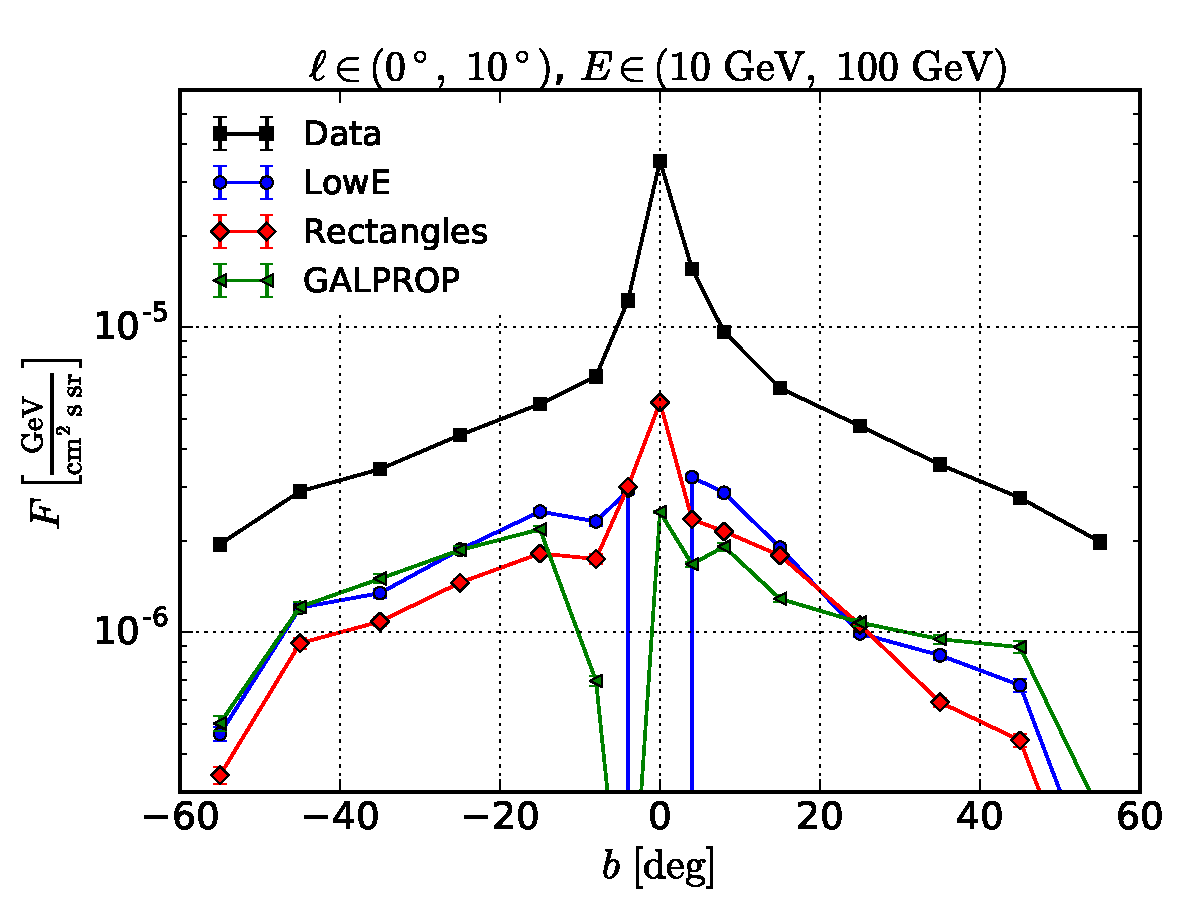
\includegraphics[width=\twopic\textwidth]{plots/Profiles_l=1_source_range_1.pdf}
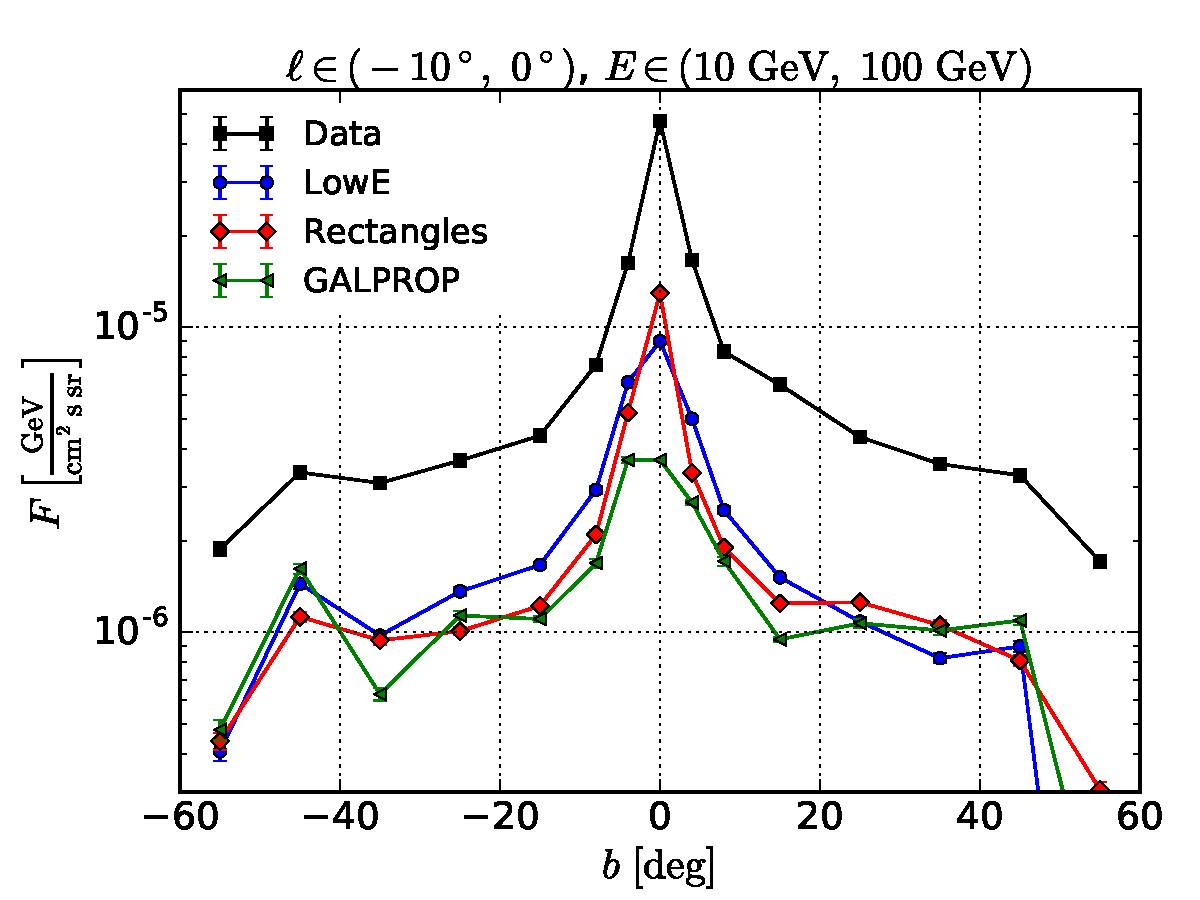
\includegraphics[width=\twopic\textwidth]{plots/Profiles_l=0_source_range_1.pdf}
  	\caption{Latitude profiles of the energy flux between 10 and 100 GeV for the total data excluding the PS mask and for 
	the FBs models for different foreground diffuse emission models to the east and to the west of the GC.}
  	\label{fig:Profiles}
\end{figure*}


\begin{figure*}[h]
\centering
%\hspace{-2mm}
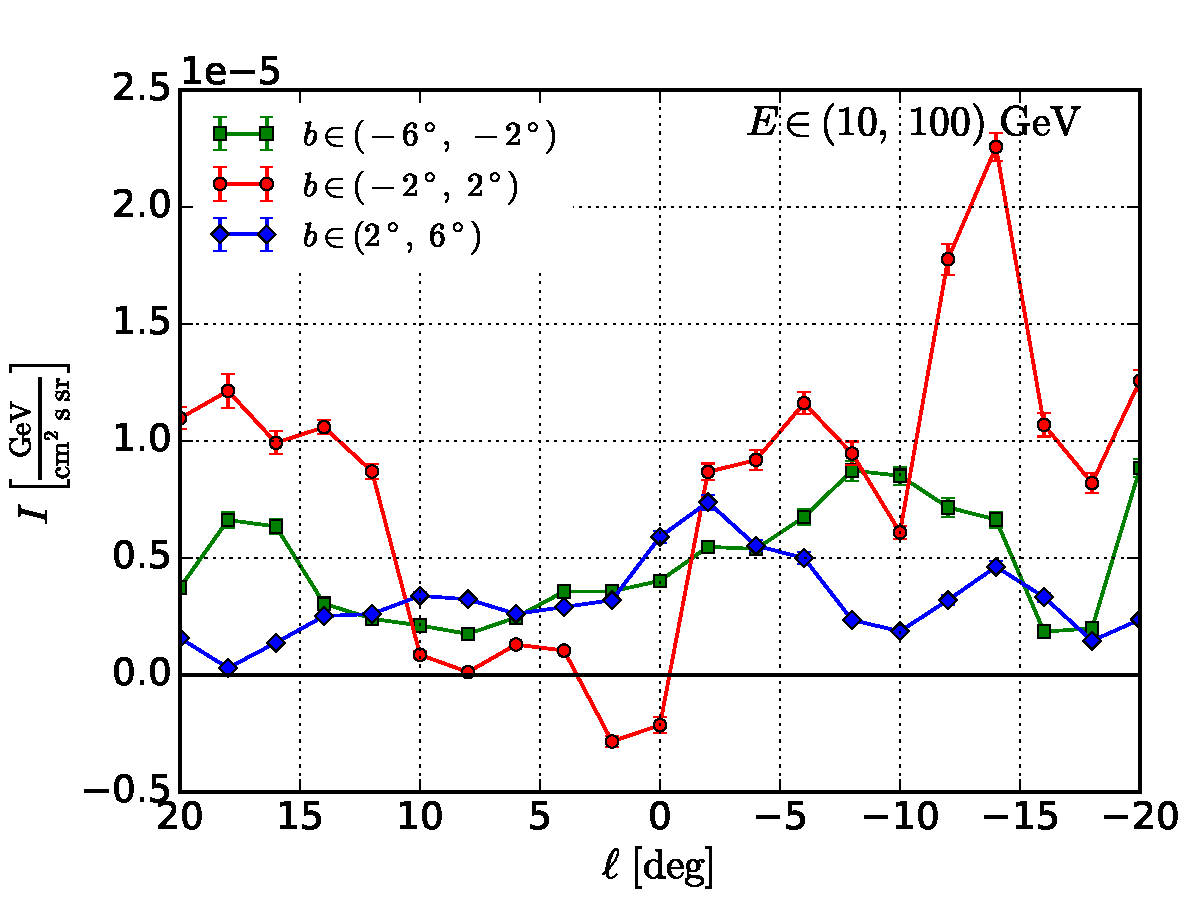
\includegraphics[width=\twopic\textwidth]{plots/Lon_profiles_LowE_source_range_1.pdf}
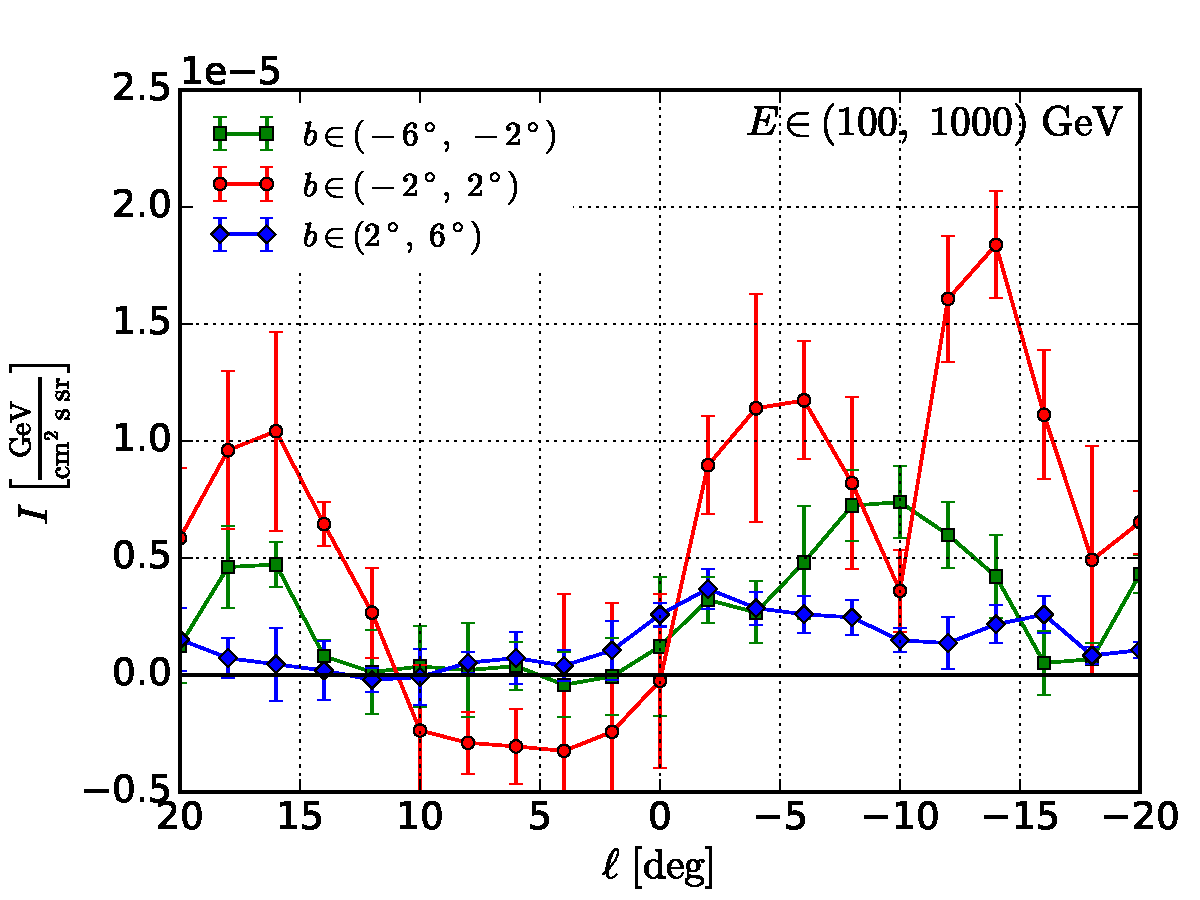
\includegraphics[width=\twopic\textwidth]{plots/Lon_profiles_LowE_source_range_2.pdf}
  	\caption{Longitude profiles of the energy flux between 10 and 100 GeV and between 100 GeV and 1 TeV 
	for the residuals in the low-energy data background model (Section \ref{sec:le_data_model}).}
  	\label{fig:lon-profiles}
\end{figure*}


\subsection{Comparison of the spectra at different latitudes}

\begin{figure*}[h]
\centering
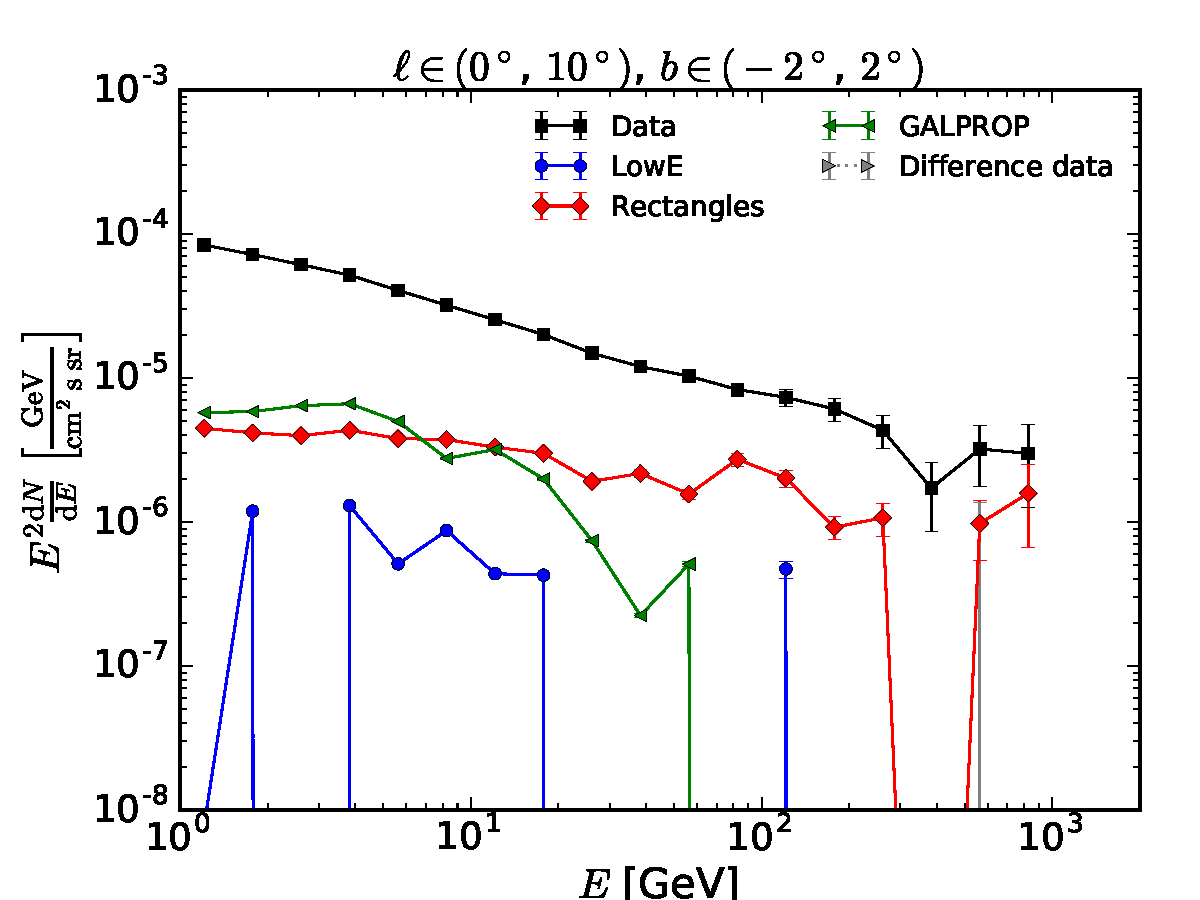
\includegraphics[width=\twopic\textwidth]{plots/SED_all_models_source_l=5_b=0.pdf}
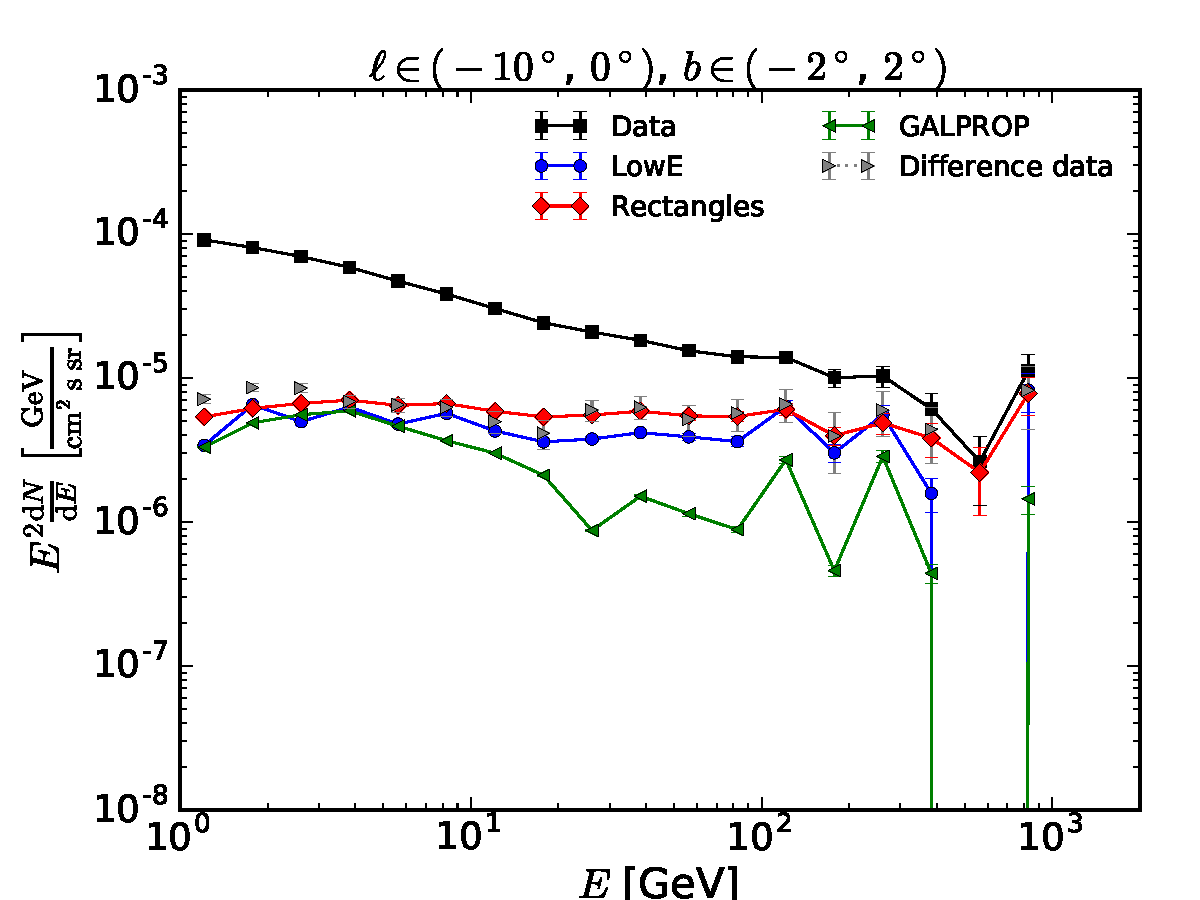
\includegraphics[width=\twopic\textwidth]{plots/SED_all_models_source_l=-5_b=0.pdf}
  	\caption{SEDs of the gamma-ray data, of the residuals (``LowE'' model), 
	rectangles model of the FBs (``rectangles'' model),
	residuals plus FBs model plus gNFW DM annihilation template (``GALPROP'' model),
	and of the difference in the data west minus east of the GC (excluding pixels in the PS mask). 
	%The width of the regions in longitude is $\ang{10}$, i.e. $\ang{0}$ to $\ang{10}$ to the east of the GC (left) and $\ang{-10}$ to $\ang{0}$ to the west of the GC (right).
	}
  	\label{fig:SED_all}
\end{figure*}

In this section we quantify the hardening of the gamma-ray spectrum at the base of the FBs. 
We first compare the spectral energy distribution (SED) of the emission at the base of the FBs for different foreground models in Figure \ref{fig:SED_all}. 
The differential flux is averaged over regions to the east, $\ell \in (\ang{0},\ \ang{10})$, and to the west, $\ell \in (\ang{-10},\ \ang{0})$, of the GC
in a thin stripe covering the Galactic plane $b \in (\ang{-2},\ \ang{2})$. 
For comparison, we show the total data (excluding pixels masked by the PS mask) and, on the plot for $\ell \in (\ang{-10},\ \ang{0})$, the difference in the data west minus east
of the GC.

For negative longitudes, all models give similar results. 
The differential flux of the GALPROP model is smaller than the differential flux of the other models above 10 GeV, 
which is consistent with the profile plots in Figure \ref{fig:Profiles}.
%We also find an asymmetry in the flux of the data with PS mask. 
The difference of the data west minus east of the GC is similar to the fluxes at the base of the FBs in the low-energy model and in the rectangles model. 
The spectra at positive longitudes show large oversubtractions and softer spectra. 
%\Laura{Should we show here the plots for (-6,-2) and (2,6) deg latitude also?}
%\dima{I'm not sure, it will take space}

To compare the behavior of the energy spectra at high energies for different latitudes, 
we fit a log-parabola plus the fixed foreground model counts to the 
total smoothed gamma-ray counts in each latitude stripe using the likelihood based on the gamma distribution.
We use the following parametrization of the log-parabola function:

 \begin{equation}
 f(E) = N_0 \left(\frac{E}{\SI{1}{GeV}}\right)^{-\alpha - \beta \ln(E / \SI{1}{GeV})}.
 \end{equation}
The local ``index'' of the spectrum at energy $E$ is

\begin{equation}
\lb{eq:log_par}
n \equiv - \frac{\de \ln f}{\de \ln E} = \alpha + 2 \beta \ln\left(\frac{E}{\SI{1}{GeV}}\right).
\end{equation}
In Figure \ref{fig:logpar_index} we show this log-parabola index $n$ as a function of latitude at $E = \SI{500}{GeV}$. 
%\Laura{You called it bubble! ;)} \dima{bubble removed}
We plot $(2 - n)$, which corresponds to the SED index.
For positive longitudes, the index is relatively soft ($n > 2$) for most of the latitudes
except high latitudes where the gamma-ray statistics are small.
For negative longitudes, the index near the GC
is significantly harder ($n \approx 2$) than the index at higher latitudes.
%\Laura{Would you like the x-axis of the log-par plot to show n-2?}
%\dima{yes, I'd suggest to put (2 - n) on the y-axis}
\begin{figure*}[h!]
\centering
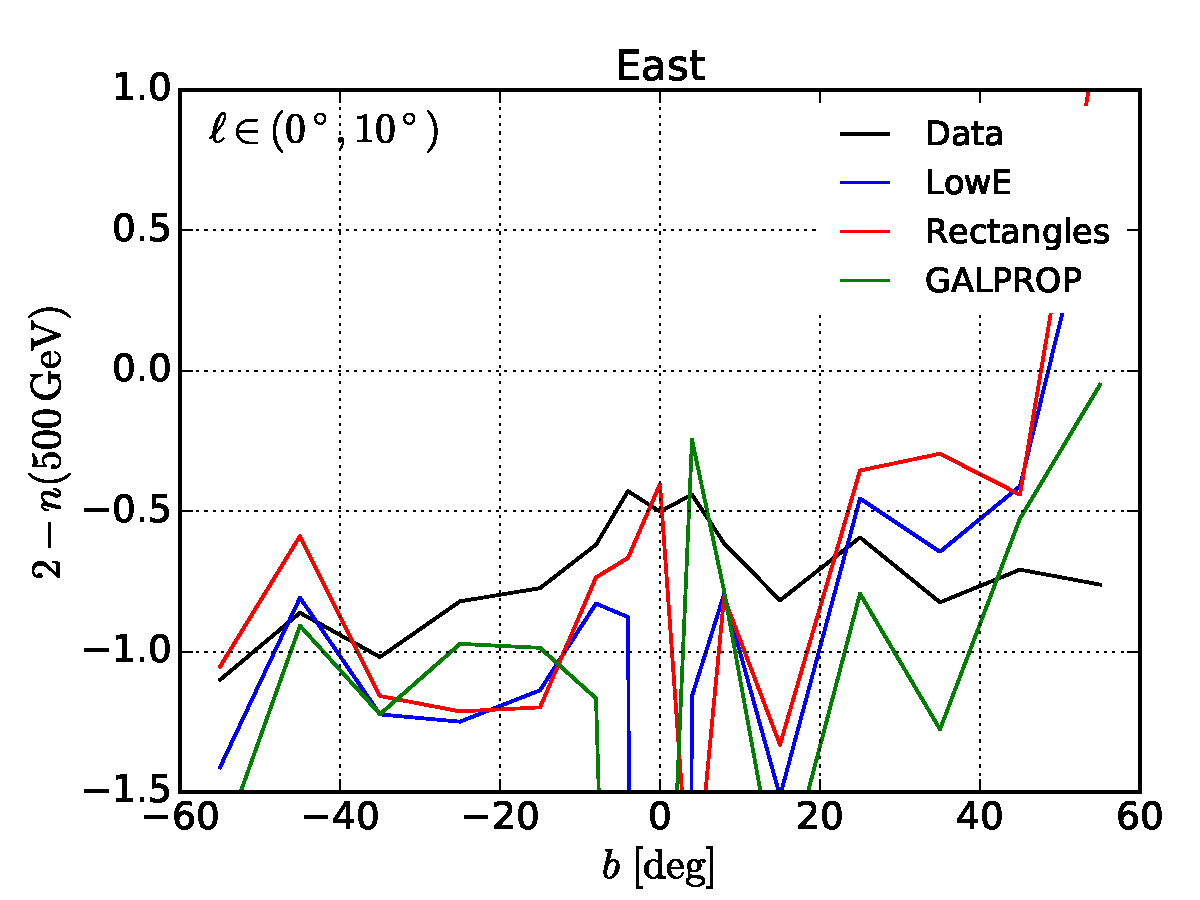
\includegraphics[width=\twopic\textwidth]{plots/LogParabola_n(500GeV)_l_in_(0,10).pdf}
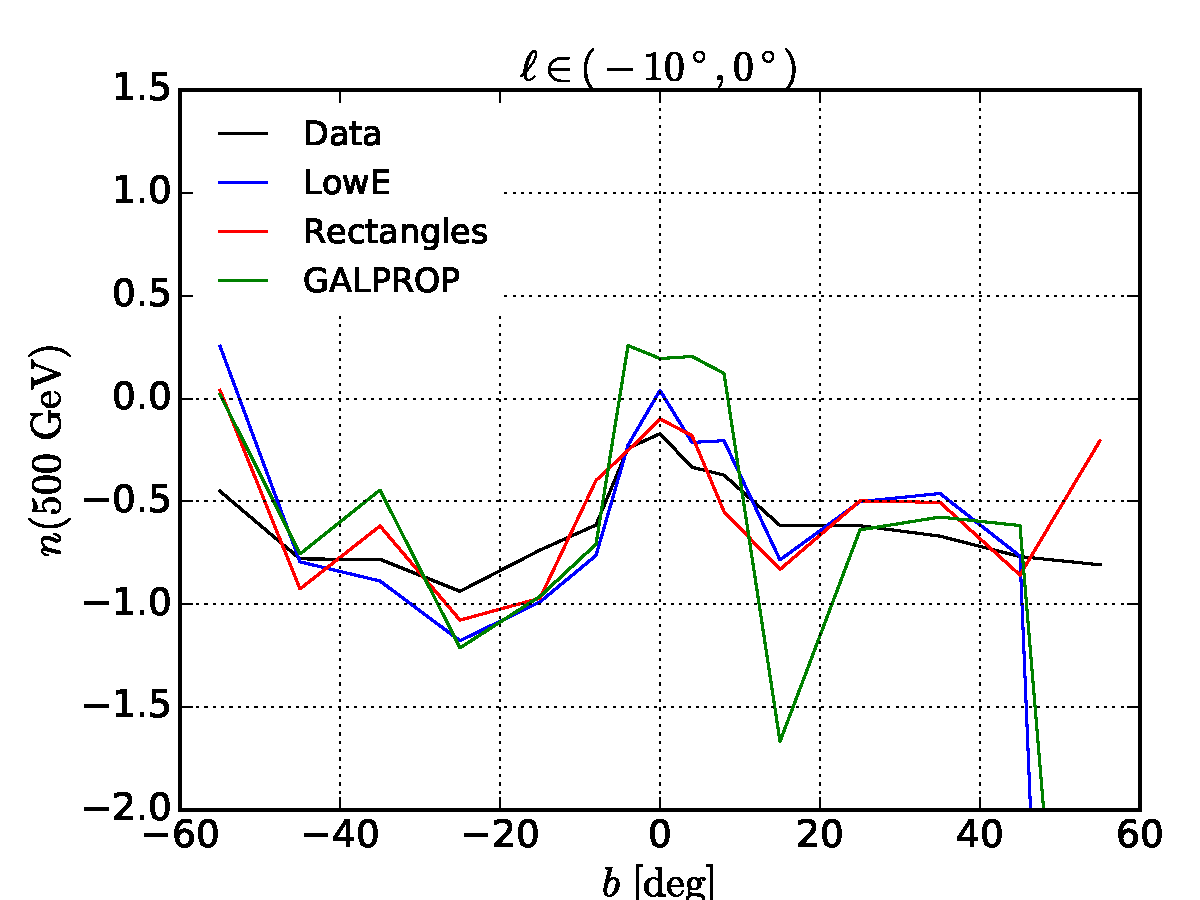
\includegraphics[width=\twopic\textwidth]{plots/LogParabola_n(500GeV)_l_in_(-10,0).pdf}
\caption{
Index of the log-parabola defined in Equation (\ref{eq:log_par}) at  $E = \SI{500}{GeV}$ as a function of latitude for the FBs in 
the different foreground diffuse emission models.
%The width of the regions in longitude is $\ang{10}$, i.e. $\ang{0} - \ang{10}$ to the east of the GC (left) and $\ang{-10} - \ang{0}$ to the west of the GC (right).
}
\label{fig:logpar_index}
\end{figure*}

% somehow we need this for latex to compile
%\vspace{2cm}
\subsection{Parametric model of the gamma-ray spectrum at low latitudes}
\label{sec:param_model}

In this section we study the spectrum at the base of the FBs at latitudes $|b| < 6^\circ$.
As a baseline model we use the rectangles model of the FBs.
We compare a power-law model of the energy spectrum with a power-law and an exponential cutoff model

\begin{equation}
\frac{dN}{dE} = N_0 \left( \frac{E}{1\:{\rm GeV}} \right)^{-n} e^{-E / E_{\rm cut}}.
\end{equation}
We fit the spectral model together with the fixed background to the total gamma-ray data counts.
The best-fit parameters for the rectangles model are reported in Table \ref{tab:param}.
If the improvement in $2 \Delta \log \La$ is less than 1, then we report the power-law model parameters
(it turns out that the improvement in $2 \Delta \log \La$ is less than 0.1 in the cases when the cutoff is not significant).
For the model with a cutoff, we also find the 95\% statistical confidence lower limit for the cutoff energy.
In the last column we report the minimum among the 95\% confidence lower limits for the three models considered in the paper
(the low-energy data model, the rectangles model, and the GALPROP templates model).
The spectrum of the residuals including the FBs at  $\ell \in (\ang{-10},\ \ang{0})$
is consistent with a power law with an index $2.1 - 2.2$ up to $E \approx 1$ TeV.
The 95\% confidence lower limit on the cutoff energy is $\sim$ 500 GeV for latitudes $|b| < 6^\circ$ within $-10^\circ < \ell < 0^\circ$.
%\dima{Report the total luminosity (assuming the GC location) in erg/s including modeling ``error bars",  we can also do it in Section \ref{sec:GC_scenario}.}

As one can see from the spectra in Figure \ref{fig:SED_all}, there are large (relative to statistical uncertainty) fluctuations in some of the models.
These fluctuations are due to modeling uncertainty of the Galactic diffuse emission.
As a result, a fit with a simple function may be sensitive to the starting point (there can be several local minima).
In the GALPROP model of the foreground, we also had to constrain the range of the index of the FB's spectrum
between 1.5 and 2.5 in the derivation of the 95\% confidence lower limit on the cutoff energy.

\begin{table*}
  \begin{center}
    \caption{Best-fit parameters of the gamma-ray spectrum and the significance of the cutoff for the rectangles model
    of the FBs.
    $E_{\rm cut, 95\%}$ is the statistical 95\% confidence lower limit on the energy cutoff of the FBs spectrum, 
    $E_{\rm cut, 95\%}^{\rm min}$ is the minimal 95\% statistical lower limit among the models of the FBs in 
    Sections \ref{sec:le_data_model} -- \ref{sec:galprop_model}.
    There are four cases when the introduction of a cutoff does not lead to improved fit: in all of these cases
    $2 \Delta \log \La < 0.1$ while the formal best-fit values of $E_{\rm cut}$ are larger than 1 TeV.
    %The numbers in parenthesis in the last two columns show the results without the last energy bin.
    %\dima{Some numbers seem to be very different with and without the last data point, e.g., 2.4 (180) and 12 (130). I've marked the strange numbers in red. Also the 95\% cutoff values for the rectangles model without the last point seem to be higher in all cases, I'd expect that they would be almost always lower.}
    %\Laura{I had normalized the powerlaw of the parametric model to 10 GeV. The correct values (for 1 GeV) are in parenthesis. IC and pi0 are not affected by the bug.}
    }
    \label{tab:param}
    \begin{tabular}{|c|c|c|c|c|c|c|c|} % <-- Alignments: 1st column left, 2nd middle and 3rd right, with vertical lines in between
     	\hline
		 Lat & Lon  & $N_0$ & $n$ & $E_{\rm cut}$ &  $2 \Delta \log \La$ & $E_{\rm cut, 95\%}$ & $E_{\rm cut, 95\%}^{\rm min}$ \\ 
		       &        &  {\small $\SI{e-6}{\rm GeV^{-1}cm^{-2}s^{-1} sr^{-1}}$ }&  & {\small $\SI{}{GeV}$ }& &{\small  $\SI{}{GeV}$ }&{\small  $\SI{}{GeV}$ }\\ 
		\hline
  		$(\ang{2}, \ang{6})$ & $(\ang{0}, \ang{10})$ & $1.5\pm 0.3$  & $1.9\pm 0.1$ & $45\pm 17$ & 4.8 & 25& 25\\ 
		& $(\ang{-10}, \ang{0})$ & $3.1 \pm 0.4$  & $2.2 \pm 0.05$  & $-$ \cmt{5.2e3} & $< 0.1$ \cmt{0.027} & {510} & {510}  \\ 
 		\hline
  		$(\ang{-2}, \ang{2})$ & $(\ang{0}, \ang{10})$  & $6.4 \pm 1.1$  & $2.3 \pm 0.09$ & $-$ \cmt{8.3e3} &  $< 0.1$ \cmt{0.010} & {300}  & {2.4}  \\ 
		& $(\ang{-10}, \ang{0})$  & $7.9 \pm 0.7$  & $2.1 \pm 0.04$ & $-$ \cmt{8.3e6} &  $< 0.1$ \cmt{3.3e-5} & {{1000}} & 600   \\ 
 		\hline
  		$(\ang{-6}, \ang{-2})$ & $(\ang{0}, \ang{10})$  & $2.5 \pm 0.4$  & $2.1 \pm 0.07$ & $260 \pm 150$ & 3.8 & 130& {2.3} \\ 
		& $(\ang{-10}, \ang{0})$ & $4.0 \pm 0.3$  & $2.2 \pm 0.04$ &  $-$ \cmt{77e3} &  $< 0.1$ \cmt{0.020} & {560}  & {560}  \\ 
 \hline
    \end{tabular}
  \end{center}
\end{table*}



\subsection{IC model of the gamma-ray emission}
\label{sec:IC_model}

In this section we model the gamma-ray emission at the base of the FBs with an IC scattering model.
The SED of the gamma-ray intensity is parametrized as

\begin{equation}
E^2_\g \frac{dF_\g}{dE_\g} = 
\frac{E_\g c}{4\pi}\int \frac{\de n_{h\nu}}{\de E_{h\nu}} \sigma_\IC\ \frac{\de \Sigma_{\el}}{\de E_{\el}} \de E_{h\nu}\, \de E_\el,
\end{equation}
where $\frac{\de \Sigma_{\el}}{\de E_{\el}} = \int \frac{\de n_{\el}}{\de E_{\el}} dR$ is the column density 
of CR electrons integrated along the line-of-sight distance $R$,
$\frac{\de n_{h\nu}}{\de E_{h\nu}}$ is the number density of ISRF photons of energy $h\nu$,
and $\sigma_\IC(E_\gamma, E_{h\nu}, E_\el)$
is the differential IC scattering cross section in units of $E_\g\frac{d\sigma}{d E_\g}$ \citep{1970RvMP...42..237B}.
For details on the parametrization of $\sigma_\IC$ see Appendix B of \cite{2014ApJ...793...64A}.
The ISRF number density for starlight and IR photons is taken from GALPROP v54 \citep{2006ApJ...640L.155M}
assuming that the emission at the base of the FBs is near the GC.
For the CMB, we use the thermal spectrum with a temperature of $\SI{2.73}{K}$.
We model the column density of electrons as a power law with a cutoff

\begin{equation} 
\label{eq:e_spectrum}
 \frac{\de \Sigma_{\el}}{\de E_{\el}} = n_\el \left(\frac{E_\el}{\SI{1}{GeV}}\right)^{-\gamma_\el} e^{- E_\el / E_{\cut}}.
\end{equation}
In order to determine the normalization $n_\el$, the spectral index $\gamma_\el$, and the cutoff  $E_{\cut}$, 
we fit the IC model of the FBs plus the (fixed) foreground model counts to the 
total smoothed gamma-ray counts in different latitude stripes using likelihood based on gamma distribution.
As a baseline case, we take the gamma-ray spectrum derived in the rectangles model of the FBs in Section \ref{sec:box_model}.
The best-fit spectra for the rectangles model of the bubbles are shown in Figure \ref{fig:SED_with_fits}
%Figure \ref{fig:SED_with_fits} shows the residual of the rectangles model within 
in latitude stripes $b \in (\ang{2}, \ang{6})$, $b \in (-\ang{2}, \ang{2})$ and $b \in (-\ang{6}, -\ang{2})$. 
%The dotted line represents the best-fit IC spectrum for an electron distribution following a simple power law.
%\Laura{Should we here compare with the spectral indices of the other models?} \dima{yes}
%The spectral index to the west of the GC of the electron spectrum is harder than the spectrum to the east of the GC. 
If the improvement in $2 \Delta \log \La$ with and without the cutoff is less than 0.1, then we show only the parameters for the power-law model without a cutoff.
For example, for negative longitudes the cutoff is not significant.

The 95\% statistical lower limit on the cutoff energy for the rectangles model and the minimum 
among the three models presented in Sections \ref{sec:le_data_model} -- \ref{sec:galprop_model}
of the 95\% confidence lower limits 
for the cutoff energy are presented in Table \ref{tab:IC}.
%We also report the 95\% lower limit on the cutoff value. 
For negative longitudes,
the 95\% confidence lower limit on the cutoff in the spectrum of electrons in the rectangles model is about 4 TeV,
while the minimal value of the 95\% confidence limit for the three models of the foreground emission is about 3 TeV.


\begin{comment}
For that, we determine the photon counts detected by \Fermi-LAT that correspond to the IC radiation generated by the electrons in the respective region. For a volume $V$ and a distance $R$ to the region, the detected counts per energy bin $E$ are 
\begin{equation}
N_{\gamma,\IC}(E) = \left(E\frac{\de n}{\de E}\right)_{\!\!\gamma,\IC} \cdot V \frac{\tau(E_\gamma)}{4 \pi R^2} \cdot \de(\log E_\gamma),
\end{equation}
where $ \de(\log E_\gamma)$ is the logarithmic size of the energy bin. Since the exposure $\tau(E_\gamma)$, which is averaged over the area on the sky, depends on energy, it can affect the shape of the electron spectrum. The quantities $V$ and $R$ only affect the normalization of the electron spectrum and will not be important until section \ref{sec:Interpretation}.
The model for the total detected counts is the sum of one of the foreground models and the counts generated by the electron density via IC scattering. As our baseline model for the foreground, we pick the rectangles model.
 We fit our model of the total counts to the actually observed total counts in that region (with PS mask) using Poisson likelihood and extract the parameters $n_\el$ and $\gamma_\el$ of the electron spectrum.
\end{comment}


\begin{comment}
For $b \in (\ang{2}, \ang{6})$ the spectral index varies between 2.92 and 3.15 for the three models, for $b \in (-\ang{2}, \ang{2})$ between 2.68 and 3.54 and for $b \in (-\ang{6}, -\ang{2})$ between 2.85 and 3.00. The softest spectrum in each latitude stripe is fitted to the GALPROP model. To the east of the GC the spectral indices vary between 2.97 and 5.09 in the three latitude stripes. 

In order to test the presence of a cutoff in the spectrum of electrons, we fit the gamma-ray data using a spectrum of the electrons
with an additional cutoff factor $\exp(-\alpha E_\el)$, where $\alpha = E^{-1}_{\el,\cut}$ is the inverse cutoff.
The improvement in the $-2 \log \La$ \dima{We use Poisson log likelihood, right? I think it will be less confusing to use $-2 \log \La$,
which we actually calculate, rather  than $\chi^2$. We could even replace the two $\chi^2$ columns in the tables with a single column $2 \Delta \log \La$,
since the actual values of $-2 \log \La$ do not mean much.}
for the models with and without the cutoff is shown in Table \ref{tab:IC}
for different latitude stripes.
\end{comment}



%We want to estimate the probability for the electron spectrum to have an exponential cutoff. For that we multiply an exponential cutoff $\exp(E_\el / E_{\el,\cut})$ to the electron spectrum \eqref{eq:e_spectrum} and determine the parameters analog to the procedure described before, using the rectangles model as the baseline foreground model.\\
%For the latitude stripe covering the Galactic plane, $b \in (-\ang{2}, \ang{2})$, adding a cutoff to the powerlaw does not improve the $\chi^2$-value both at negative ($\chi^2 \approx 135$) and positive longitudes ($\chi^2 \approx 128$).

%We determine the lower bound for the cutoff energy at a $\SI{95}{\percent}$-confidence level for our baseline model, the value in parenthesis gives the lowest value for all models: For negative longitudes we find a lower bound for the cutoff energy at $\SI{13.3}{TeV}$ ($\SI{2.9}{TeV}$), for positive longitudes at $\SI{491}{GeV}$ ($\SI{16}{GeV}$).

%Slightly below the Galactic plane, $b \in (-\ang{6}, -\ang{2})$, the $\chi^2$-value does not improve by exchanging the simple powerlaw by a powerlaw with a cutoff at negative longitudes ($\chi^2 \approx 76$). At positive longitudes the $\chi^2$-value improves slightly by adding the cutoff ($\chi^2 = 98$ to $\chi^2 = 87$). For negative longitudes we find a lower bound for the cutoff energy at $\SI{6.89}{TeV}$ ($\SI{6.89}{TeV}$), for positive longitudes at $\SI{818}{GeV}$ ($\SI{0.79}{GeV}$), at a $\SI{95}{\percent}$-confidence level.

\begin{figure}[h!]
\centering
%\hspace{-2mm}
%\begin{comment}
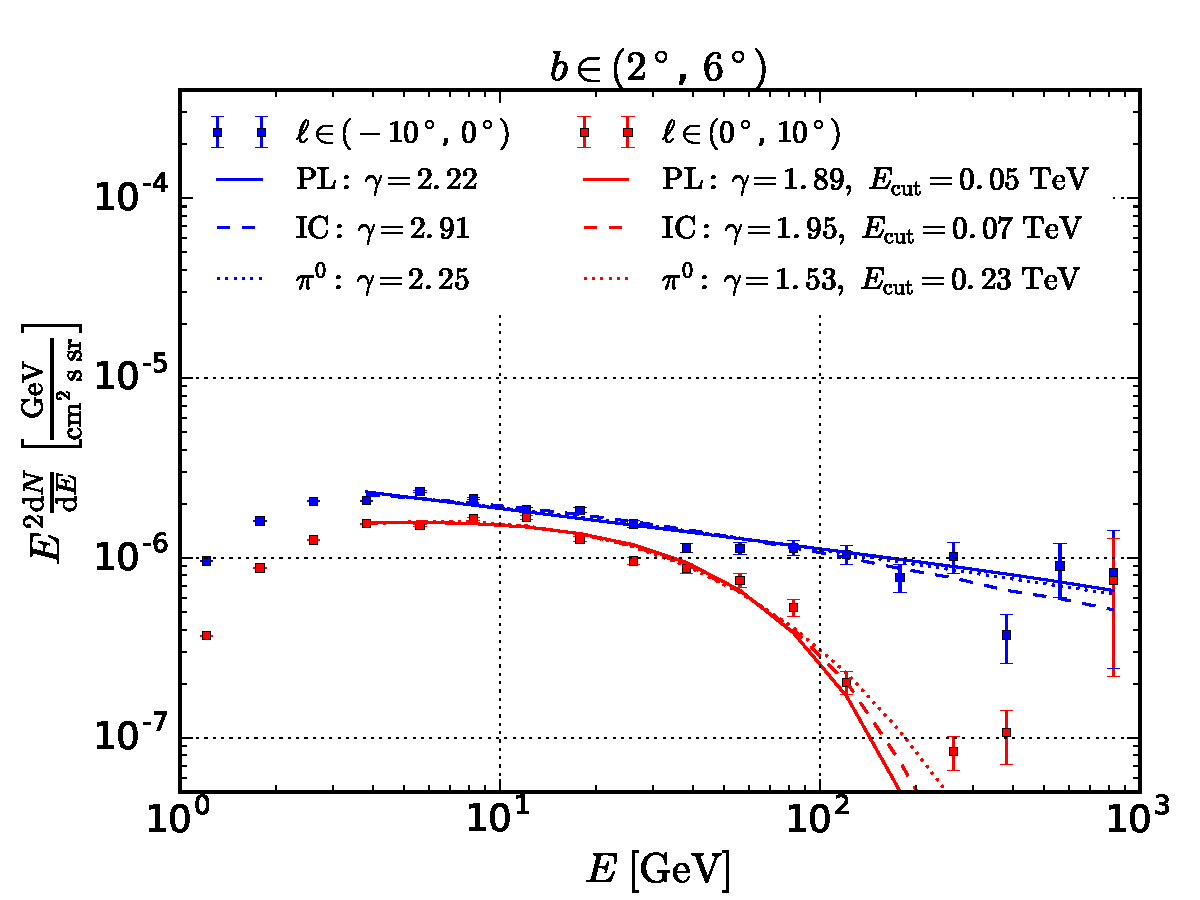
\includegraphics[width=\onepic\textwidth]{plots/SED_boxes_source_4cutoff.pdf} \\
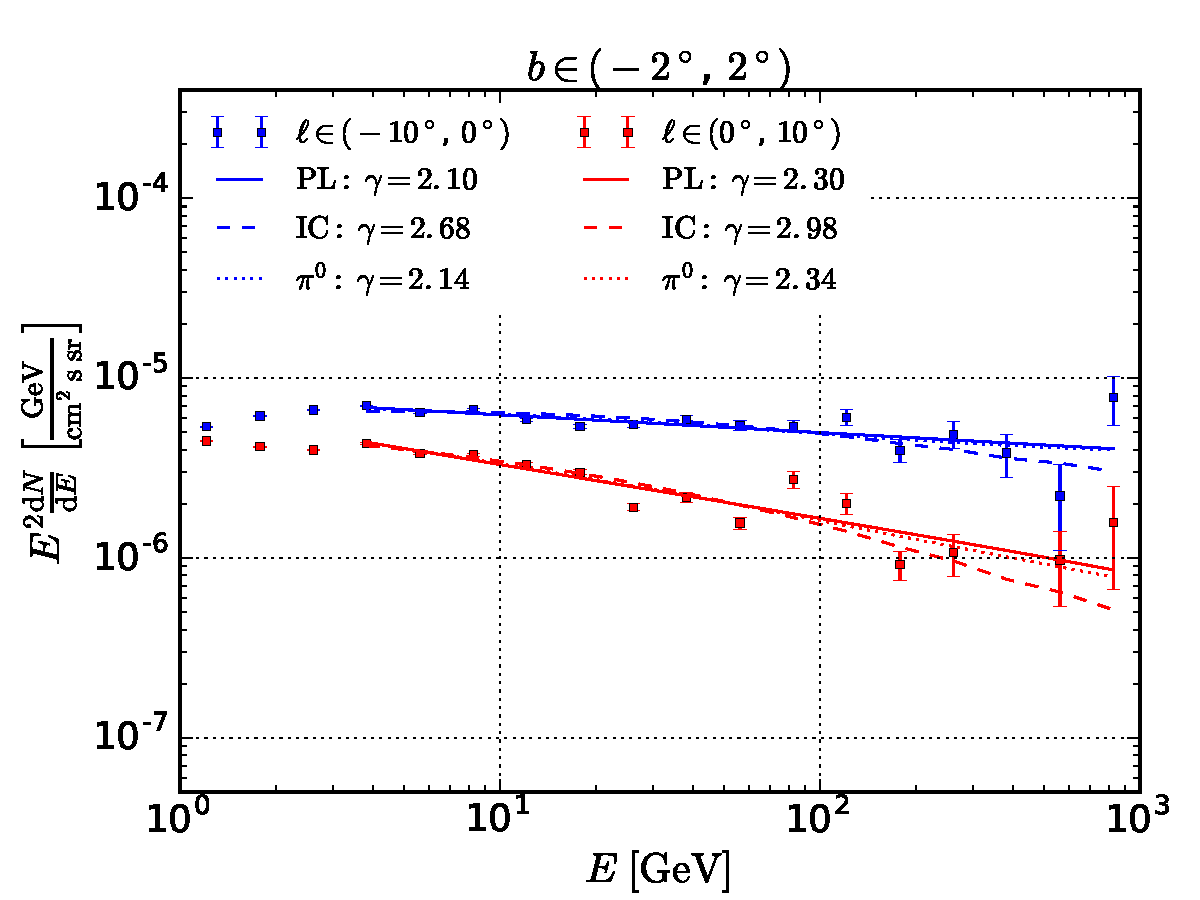
\includegraphics[width=\onepic\textwidth]{plots/SED_boxes_source_0cutoff.pdf} \\
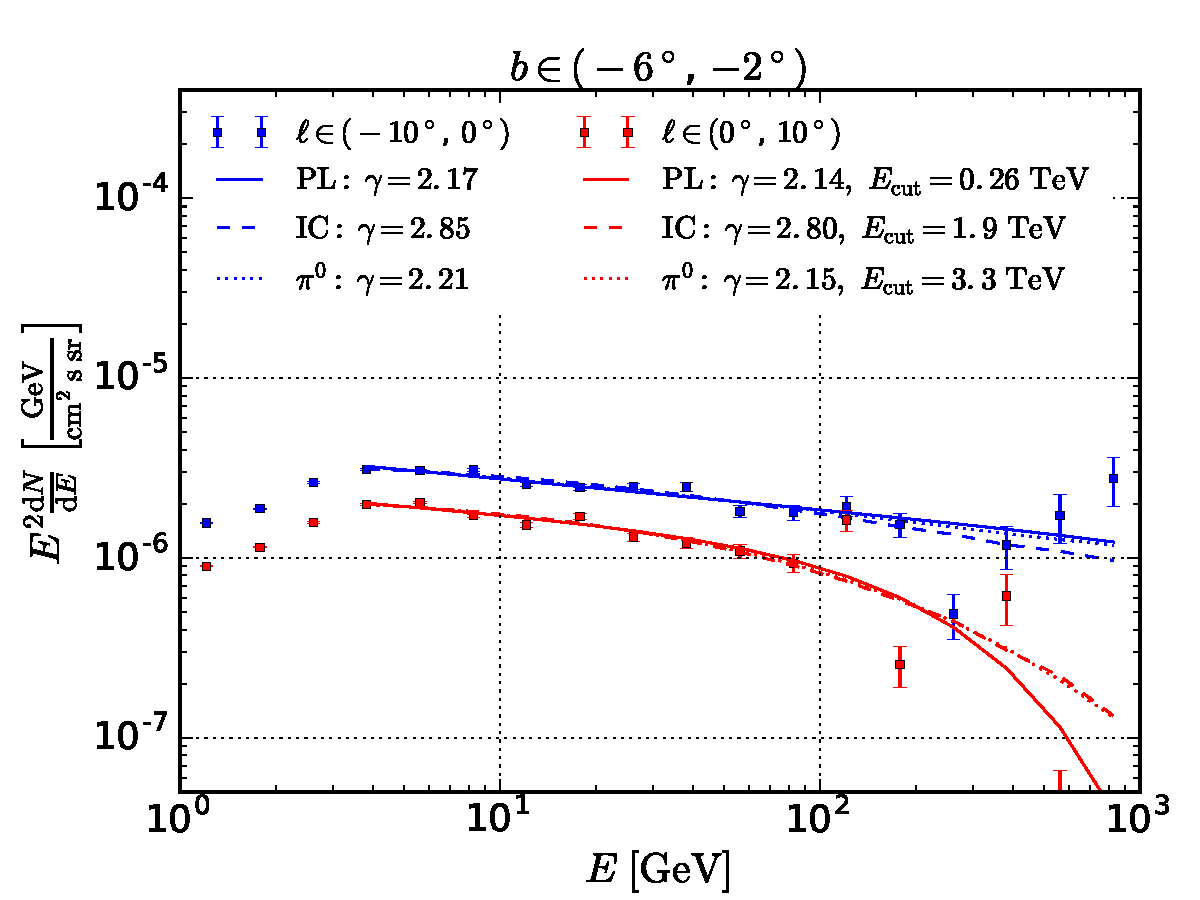
\includegraphics[width=\onepic\textwidth]{plots/SED_boxes_source_-4cutoff.pdf}
%\end{comment}
  	\caption{SEDs of the rectangles model of the FBs in the latitude stripes $(\ang{2}, \ang{6})$, $(\ang{-2}, \ang{2})$ and $(\ang{-6}, \ang{-2})$ for negative (blue) and positive (red) longitudes. We compare the parametric model of the SED with the leptonic (Section \ref{sec:IC_model}) 
	and the hadronic (Section \ref{sec:Pion_model}) models.}
  	%\Laura{Should we add the spectrum for the latitude band $(\ang{2}, \ang{6})$ also, or just say that it looks similar?}
	%\blue{Dima: yes, let's add the 2 to 6 deg spectrum.}
  	\label{fig:SED_with_fits}
\end{figure}

%
%\begin{center}
%\begin{tabular}{ |c|c|c|c|c| } 
% \hline
% lat & lon  & $\chi^2$(no cutoff) &  $\chi^2$(cutoff) & Lower bound $E_\cut$ \\ 
% \hline
%  2 -- 6 & east & $\chi^2$(no cutoff) &  $\chi^2$(cutoff) & Lower bound $E_\cut$\\ 
%2 -- 6 & west & $\chi^2$(no cutoff) &  $\chi^2$(cutoff) & Lower bound $E_\cut$ \\ 
% \hline
%   -2 -- 2 & east & $\chi^2$(no cutoff) &  $\chi^2$(cutoff) & Lower bound $E_\cut$\\ 
%-2 -- 2 & west & $\chi^2$(no cutoff) &  $\chi^2$(cutoff) & Lower bound $E_\cut$\\ 
% \hline
%  -6 -- -2 & east & $\chi^2$(no cutoff) &  $\chi^2$(cutoff) & Lower bound $E_\cut$\\ 
%-6 -- -2 & west & $\chi^2$(no cutoff) &  $\chi^2$(cutoff) & Lower bound $E_\cut$\\ 
% \hline
%\end{tabular}
%\end{center}

\begin{table*}
  \begin{center}
    \caption{Energy cutoff values and the significance of the cutoff in the IC model of the FBs at low latitudes.
%  $\chi^2$-values for IC-spectrum fit of a distribution of electrons following a simple powerlaw and a powerlaw with cutoff, respectively in the latitude bands discussed in the text. 
The lower bounds for $E_\cut$ at the 95\% confidence level for our baseline model and the minimum among the models 
presented in Sections \ref{sec:le_data_model} -- \ref{sec:galprop_model}
are shown in the last two columns respectively.
}
    \label{tab:IC}
    \begin{tabular}{|c|c|c|c|c|} % <-- Alignments: 1st column left, 2nd middle and 3rd right, with vertical lines in between
     	\hline
		 Lat & Lon  & $2 \Delta \log \La$ & \multicolumn{2}{c|}{Lower bound on $E_\cut$ (TeV) } \\ 
		       &        &                                  &  \multicolumn{1}{c}{Rectangles model} & All models \\ 
		\hline
  		$(\ang{2}, \ang{6})$ & $(\ang{0}, \ang{10})$ & 2.6  & {0.20} & {0.17}\\ 
		& $(\ang{-10}, \ang{0})$ & $ < 0.1$  & 4.0  & 4.0 \\ 
 		\hline
  		$(\ang{-2}, \ang{2})$ & $(\ang{0}, \ang{10})$ & $ < 0.1$ & {1.4} & 0.01 \\ 
		& $(\ang{-10}, \ang{0})$ & $ < 0.1$ & 13  & 2.9  \\ 
 		\hline
  		$(\ang{-6}, \ang{-2})$ & $(\ang{0}, \ang{10})$ & 1.1 & {0.82} & 0.03 \\ 
		& $(\ang{-10}, \ang{0})$& $ < 0.1$ & {7.0} & {7.0} \\ 
 \hline
    \end{tabular}
  \end{center}
\end{table*}




%\begin{figure}
%	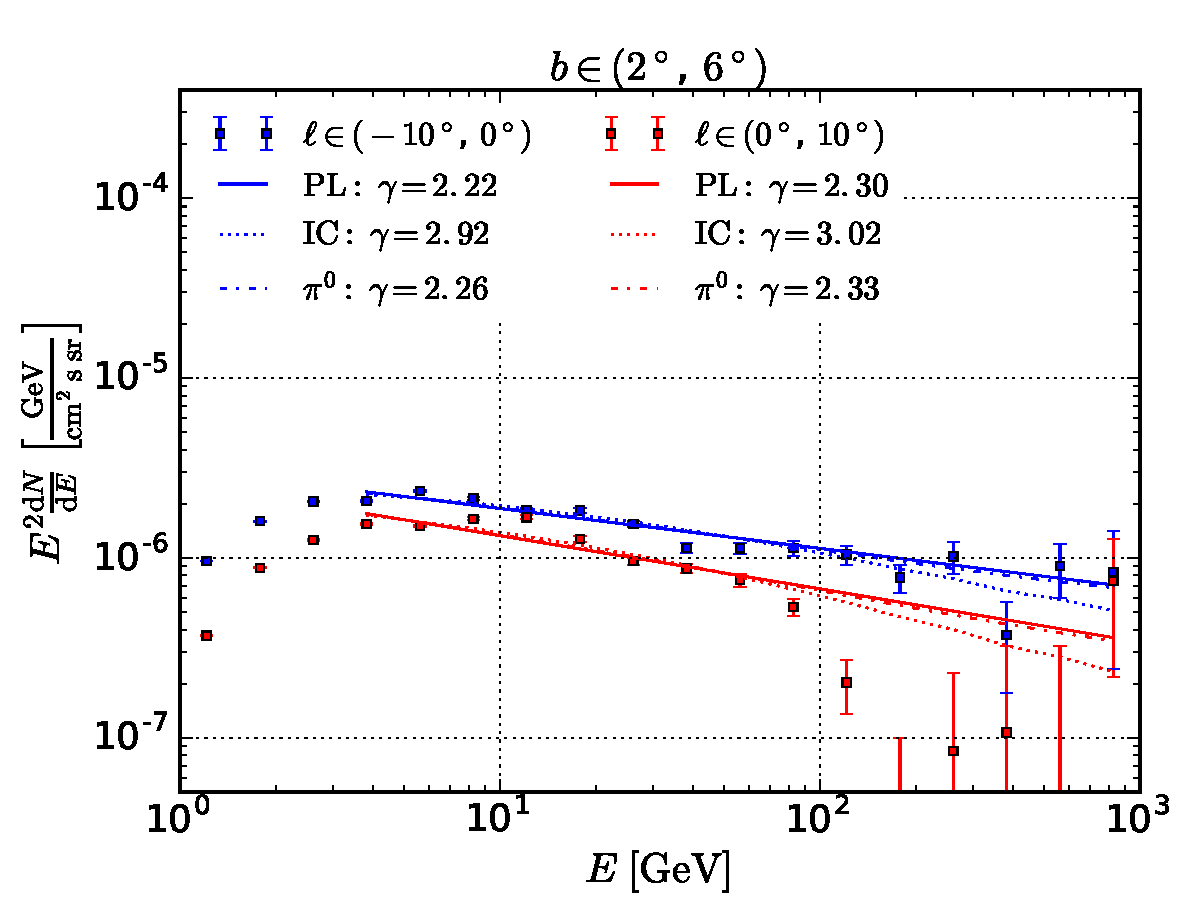
\includegraphics[width=0.5\textwidth]{plots/SED_boxes_source_4.pdf}
%\end{figure}
%\begin{figure}
%	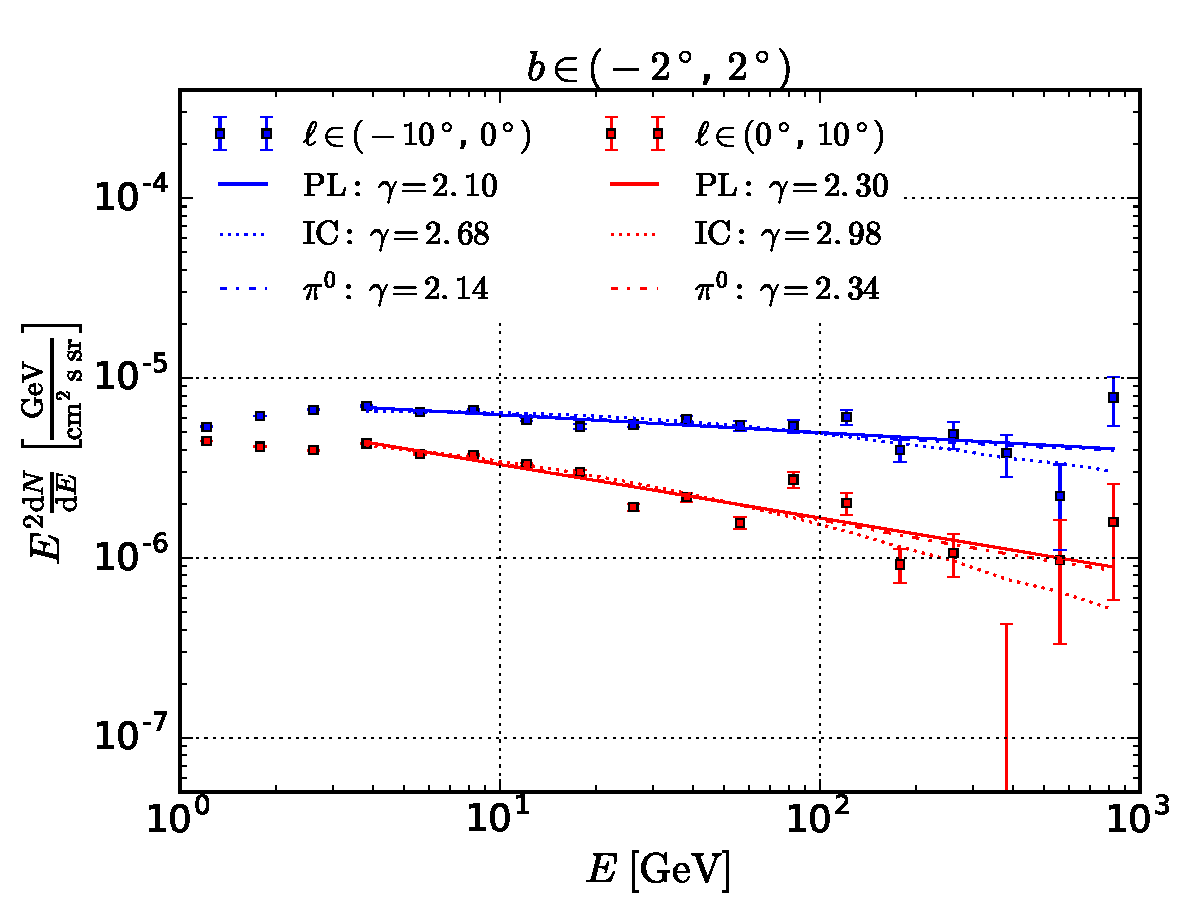
\includegraphics[width=0.5 \textwidth]{plots/SED_boxes_source_0.pdf}
%\end{figure}
%\begin{figure}
%	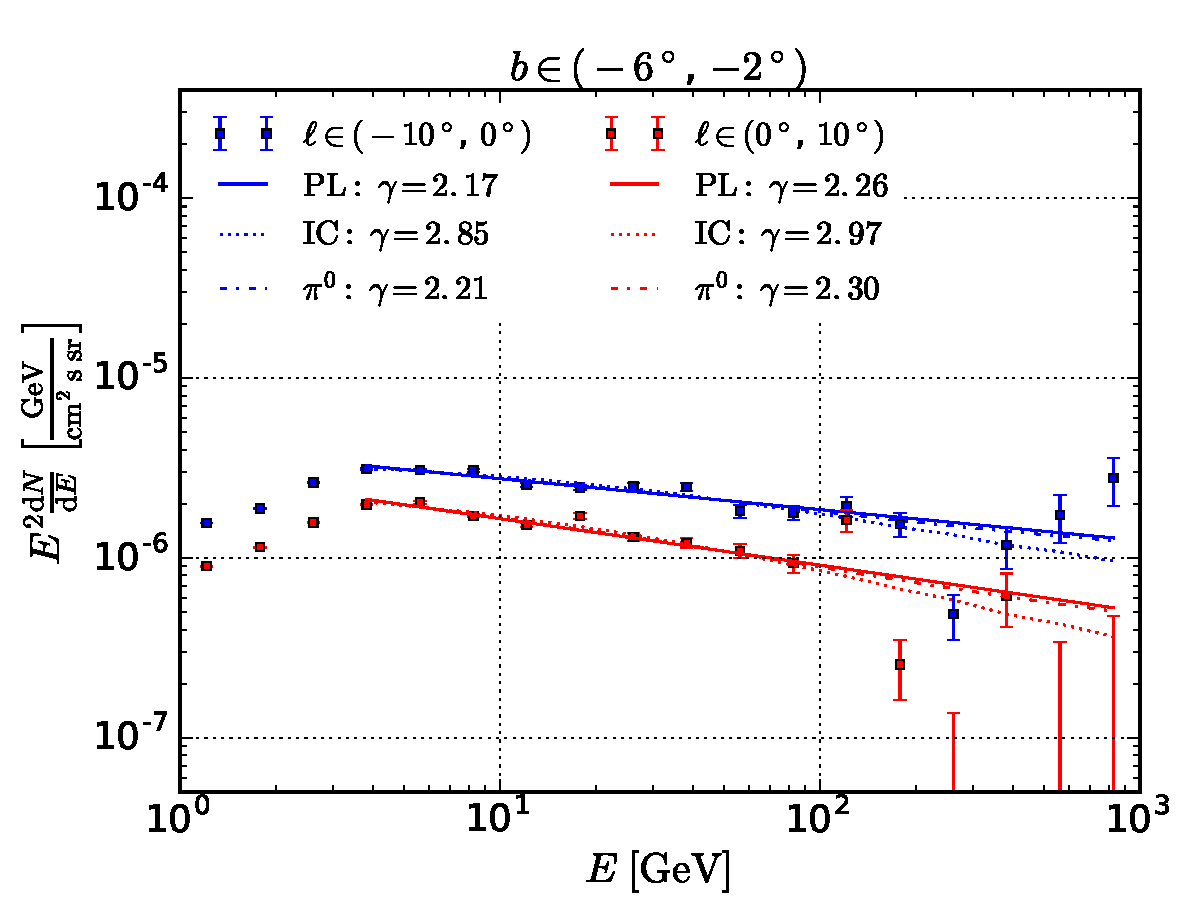
\includegraphics[width=0.5\textwidth]{plots/SED_boxes_source_-4.pdf}
%	\caption{SED of rectangles-model residual in the latitude stripes $(\ang{-2}, \ang{2})$ (left) and $(\ang{-6}, \ang{-2})$ (right) for negative (blue) and positive longitudes (red). We determine the spectral index of a powerlaw (PL), of an electron distribution emitting gamma-rays via IC and of a proton distribution emitting gamma-rays via $\pi^0$-decay.}
%\end{figure}


\subsection{Hadronic model of gamma-ray emission}
\label{sec:Pion_model}

In the hadronic model, the gamma rays are produced as a result of collisions of hadronic CR with the interstellar gas.
The gamma-ray intensity in the hadronic model is parametrized as

\be
E^2_\g \frac{dF_\g}{dE_\g} = \frac{E_\g}{4\pi} \int n_\Hy\ \sigma_\pr v_\pr \left(\frac{\de \Sigma}{\de T}\right)_{\!\!\pr} \de T_\pr,
\ee
where $\left(\frac{\de \Sigma}{\de T}\right)_{\!\!\pr} = \int \left(\frac{\de n}{\de T}\right)_{\!\!\pr} dR$ is the column density 
of CR protons, $v_\pr$ is the velocity of the protons,
$T_\pr = \sqrt{(q c)^2 + (m_p c^2)^2} - m_p c^2$ is the kinetic energy of the protons as a function of momentum $q$,
$\sigma_\pr (E_\gamma, T_\pr)$ is 
the differential cross section in units of $E_\g\frac{d\sigma}{d E_\g}$
for gamma rays in proton-proton collisions \citep{2006ApJ...647..692K, 2008ApJ...674..278K},
and $n_\Hy$ is the density of gas.
We will use $n_\Hy = \SI{1}{cm^{-3}}$ as a reference density,
which is comparable with the gas surface density of $\sim 30 M_\odot {\rm pc}^{-2}$ \citep{2017ApJ...834...57M}
averaged over the approximate height of the enhanced emission at the base of the bubbles, e.g., $\sim 900$ pc above and below the GC.
Since most of the gas density is concentrated within 100 -- 200 pc from the midplane \citep[e.g.,][]{2013pss5.book..985S, 2017ApJ...834...57M},
the gas density in the plane near the GC is 5 -- 10 ${\rm cm^{-3}}$, which is consistent with the enhancement of the intensity of the emission
at the base of the FBs at $\ell = 0^\circ$.
We model the proton spectrum as a power law of the momentum $\frac{d \Sigma}{d qc} = n_\pr q^{-\g_p}$ 
(note, that $ v_\pr \frac{\de \Sigma}{\de T_\pr} = c \frac{d \Sigma}{d qc}$).

We fit the hadronic model of the gamma-ray emission at the base of the FBs analogously to the leptonic model in 
Section \ref{sec:IC_model}.
%We add the hadronic model of the gamma-ray emission at the base of the FBs to the foreground emission 
%and determine the normalization $n_\pr$ and index $\gamma_\pr$ of the CRp spectrum
%by fitting the total model to the \Fermi-LAT data using Poisson log likelihood.
The dash-dotted line in Figure \ref{fig:SED_with_fits} represents the best-fit hadronic spectrum (labeled as $\pi^0$). 
The index of the proton spectrum is relatively hard $\g_\pr \lesssim 2.3$, especially to the west of the GC.
\begin{comment}
For that, we again fit the sum of the photon counts generated by hadronic processes and the baseline model for the foreground to the total photon counts detected by the \Fermi-LAT (with PS mask) using Poisson likelihood.  
For $b \in (\ang{2}, \ang{6})$ the spectral index to the west of the GC varies between 2.26 and 2.42, for $b \in (-\ang{2}, \ang{2})$ between 2.14 and 2.64 and for $(-\ang{6}, -\ang{2})$ between 2.21 and 2.32. To the east of the GC the indices vary between 2.33 and 3.55. 
\end{comment}

We calculate the significance of a cutoff in the CR proton spectrum by adding an exponential cutoff factor and refitting the model to the gamma-ray data.
The improvement in the model and the 95\% confidence lower bound on the cutoff values are presented in Table \ref{tab:pi0}.
Within $\pm 6^\circ$ from the Galactic plane west of the GC, the 95\% confidence level for the lower bound on the cutoff among the models
of the foreground emission that we have considered in Sections \ref{sec:le_data_model} -- \ref{sec:galprop_model} is about 6 TeV.


\begin{comment}
We again estimate the probability for the proton spectrum to have an exponential cutoff: For the latitude stripe covering the Galactic plane, $b \in (-\ang{2}, \ang{2})$, adding a cutoff does neither improve the $\chi^2$-valueat negative ($\chi^2 \approx 62$) nor positive longitudes ($\chi^2 \approx 116$). At a $95\%$-confidence level, the lower bound for the cutoff energy for the baseline model (and all models) is $\SI{28.6}{TeV}$ ($\SI{22.6}{TeV}$) for negative longitudes and $\SI{1.8}{TeV}$ ($\SI{11.5}{GeV}$) for positive longitudes.\\
In the latitude band $(-\ang{6}, -\ang{2})$, the $\chi^2$-value does increase both for negative ($\chi^2 = 157$ to $\chi^2 = 123$) and positive longitudes ($\chi^2 = 245$ to $\chi^2 = 156$) by adding an exponential cutoff. The lower bound on the cutoff energy is $\SI{23.6}{TeV}$ ($\SI{0.99}{TeV}$) for negative and $\SI{1.57}{TeV}$ ($\SI{40}{GeV}$) for positive longitudes.
\end{comment}


\begin{table*}
  \begin{center}
    \caption{\label{tab:pi0} 
Energy cutoff values and the significance of the cutoff in the hadronic model of the FBs at low latitudes.
%    $\chi^2$-values for hadronic-spectrum fit of a distribution of protons following a simple powerlaw and a powerlaw with a cutoff, respectively in the latitude bands discussed in the text. 
The lower bounds for $E_\cut$ at the 95\% confidence level for our baseline model and the minimum 
among the models presented in Sections \ref{sec:le_data_model} -- \ref{sec:galprop_model}
 are shown in the last two columns respectively. 
}
    \begin{tabular}{|c|c|c|c|c|} % <-- Alignments: 1st column left, 2nd middle and 3rd right, with vertical lines in between
     	\hline
		 lat & lon  & $2 \Delta \log \La$ & \multicolumn{2}{c|}{Lower bound on $E_\cut$ (TeV) } \\
		      &        &                                  &       \multicolumn{1}{c}{Rectangles model} & All models \\ 
		\hline
  		$(\ang{2}, \ang{6})$ & $(\ang{0}, \ang{10})$ & 4.4 & {0.88} & {0.48} \\ 
		& $(\ang{-10}, \ang{0})$ &  $ < 0.1$ & {7.4} & {7.4}\\ 
 		\hline
  		$(\ang{-2}, \ang{2})$ & $(\ang{0}, \ang{10})$ & $ < 0.1$ & {3.8} & 0.023 \\ 
		& $(\ang{-10}, \ang{0})$ & $ < 0.1$ & {29} & 6.3 \\ 
 		\hline
  		$(\ang{-6}, \ang{-2})$ & $(\ang{0}, \ang{10})$ & 2.7 & 1.6 & 0.05 \\ 
		& $(\ang{-10}, \ang{0})$ & $ < 0.1$ & {12} & {12}\\ 
 \hline
    \end{tabular}
  \end{center}
\end{table*}

\subsection{Summary of the spectral analysis}

In Figure \ref{fig:spec_summary} we show the envelopes of the gamma-ray spectra at $|b| < 2^\circ$ of the emission at the base of the FBs
for the models of foreground emission that we have considered, including the models where we change the selection of the low energies 
in the definition of the foreground emission model (Appendix \ref{sec:lowE_syst}).
In order to determine the maximal and minimal models of the FBs in the Galactic plane, 
we fit the maximal and minimal points in the envelope above 3 GeV with a power law with a cutoff function
(we fit above 3 GeV because some of the models of the foreground emission in Appendix \ref{sec:lowE_syst} are determined 
for energies between 1 and 2.2 GeV).
The corresponding parameters are reported in the first row of Table \ref{tab:summary}.
We also fit the IC and hadronic models to the maximal and minimal points in the envelope and report the corresponding parameters
in Table \ref{tab:summary}.


%\dima{we can put a summary plot with the baseline model and the band of all spectra in a small subsection here}

\begin{figure*}[h]
\centering
 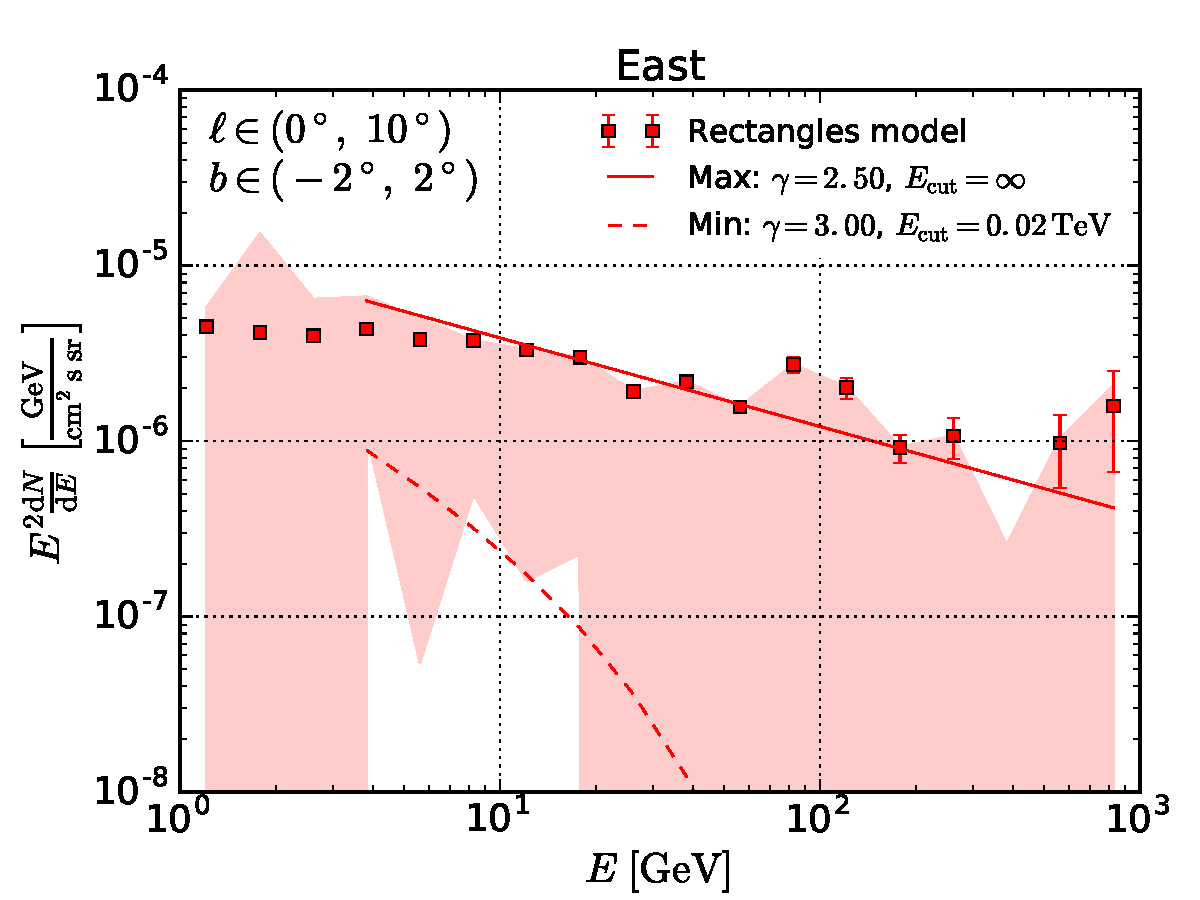
\includegraphics[width=\twopic\textwidth]{plots/Summary_SED_b=0_l=5.pdf}
  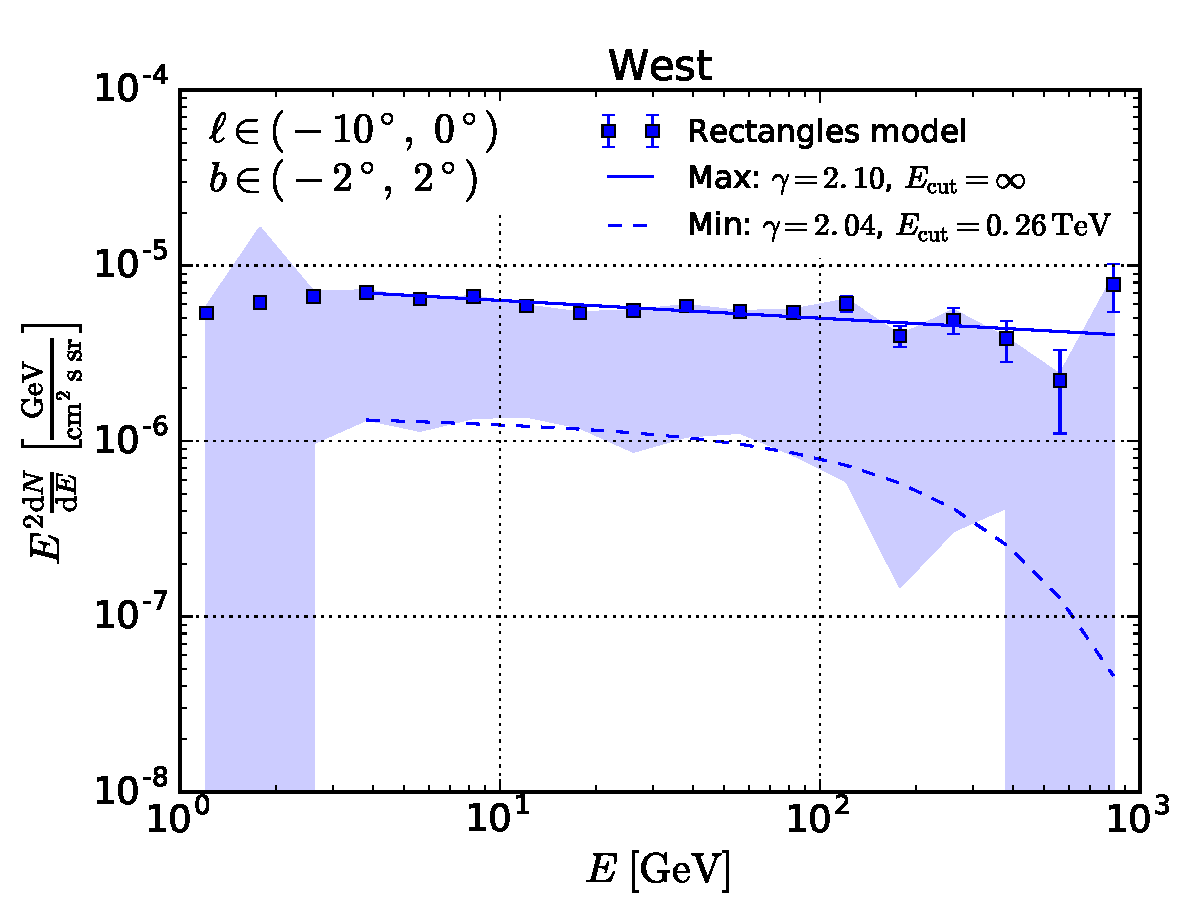
\includegraphics[width=\twopic\textwidth]{plots/Summary_SED_b=0_l=-5.pdf}
 \caption{SED of the FBs in the Galactic plane. 
 The shaded areas show the envelope of the FB's spectra in all foreground models considered in the paper
including the changes in the choice of the low-energy range to model the foreground emission
(discussed in Appendix \ref{sec:lowE_syst}).
The lines show the fits to the maximal and minimal points in the envelopes above 3 GeV.
}
 \label{fig:spec_summary}
\end{figure*}


\begin{table*}
  \begin{center}
    \caption{Summary of the min and max models for the parametric, 
    IC and hadronic models of the FBs for $|b| < 2^\circ$ and $-10^\circ < \ell < 0^\circ$. 
    For the parametric model, we report the energy spectrum of the gamma rays,
    for the IC model we report the column density of the electrons' spectrum as a function of energy,
    while for the hadronic model -- the column density of the protons' spectrum as a function of momentum.
    The spectra are normalized at $E_0 = 1$ GeV. The last column shows the statistical 95\% confidence lower limit on the cutoff, $E_{\rm cut, 95\%}$.}
    \label{tab:summary}
    \begin{tabular}{| l |c|c|c|c|c|c|c|} % <-- Alignments: 1st column left, 2nd middle and 3rd right, with vertical lines in between
     	\hline
		 {\hspace{2cm}Model} & Type  & norm & index & cutoff & $E_{\rm cut, 95\%}$ \\ 
		       &        &   &  & {\rm\small TeV} & {\rm\small TeV}\\ 
		\hline
  		\multirow{2}{*}{Parametric, $\frac{dN_\g}{dE}$ {\small $\left[{\rm {GeV^{-1}\, cm^{-2}\, s^{-1} }}\right]$}} & max &  $\SI{7.8e-6}{}$ \red{}& 2.09 \red{} &  -- & 0.99 \red{} \\ 
		& min & $\SI{1.4e-6}{}$ \red{}& 2.01 \red{} & 0.16 \red{} & 0.04 \red{} \\ 
 		\hline
  		\multirow{2}{*}{IC, $\frac{d\Sigma_e}{dE}$ {\small $\left[{\rm {GeV^{-1}\, cm^{-2}}}\right]$}} & max & $\SI{3.4e10}{}$ & 2.67 &  -- & 19 \\ 
		& min & $\SI{1.3e10}{}$ & 2.81 &  7.2 & 0.96 \\ 
 		\hline
  		\multirow{2}{*}{Hadronic, $\frac{d\Sigma_p}{dqc}$ {\small $\left[{\rm {GeV^{-1}\, cm^{-2}}}\right]$}} & max & $\SI{9.5e11}{}$ & 2.13 &  -- &65 \\ 
		& min & $\SI{1.1e11}{}$ & 1.98 &  1.8 & 0.23  \\ 
 \hline
    \end{tabular}
  \end{center}
\end{table*}



